\section{Experiments and Comparisons}\label{experiments}

\begin{figure*}[Ht!]
\centering
\begin{minipage}[t]{.49\textwidth}
\centering
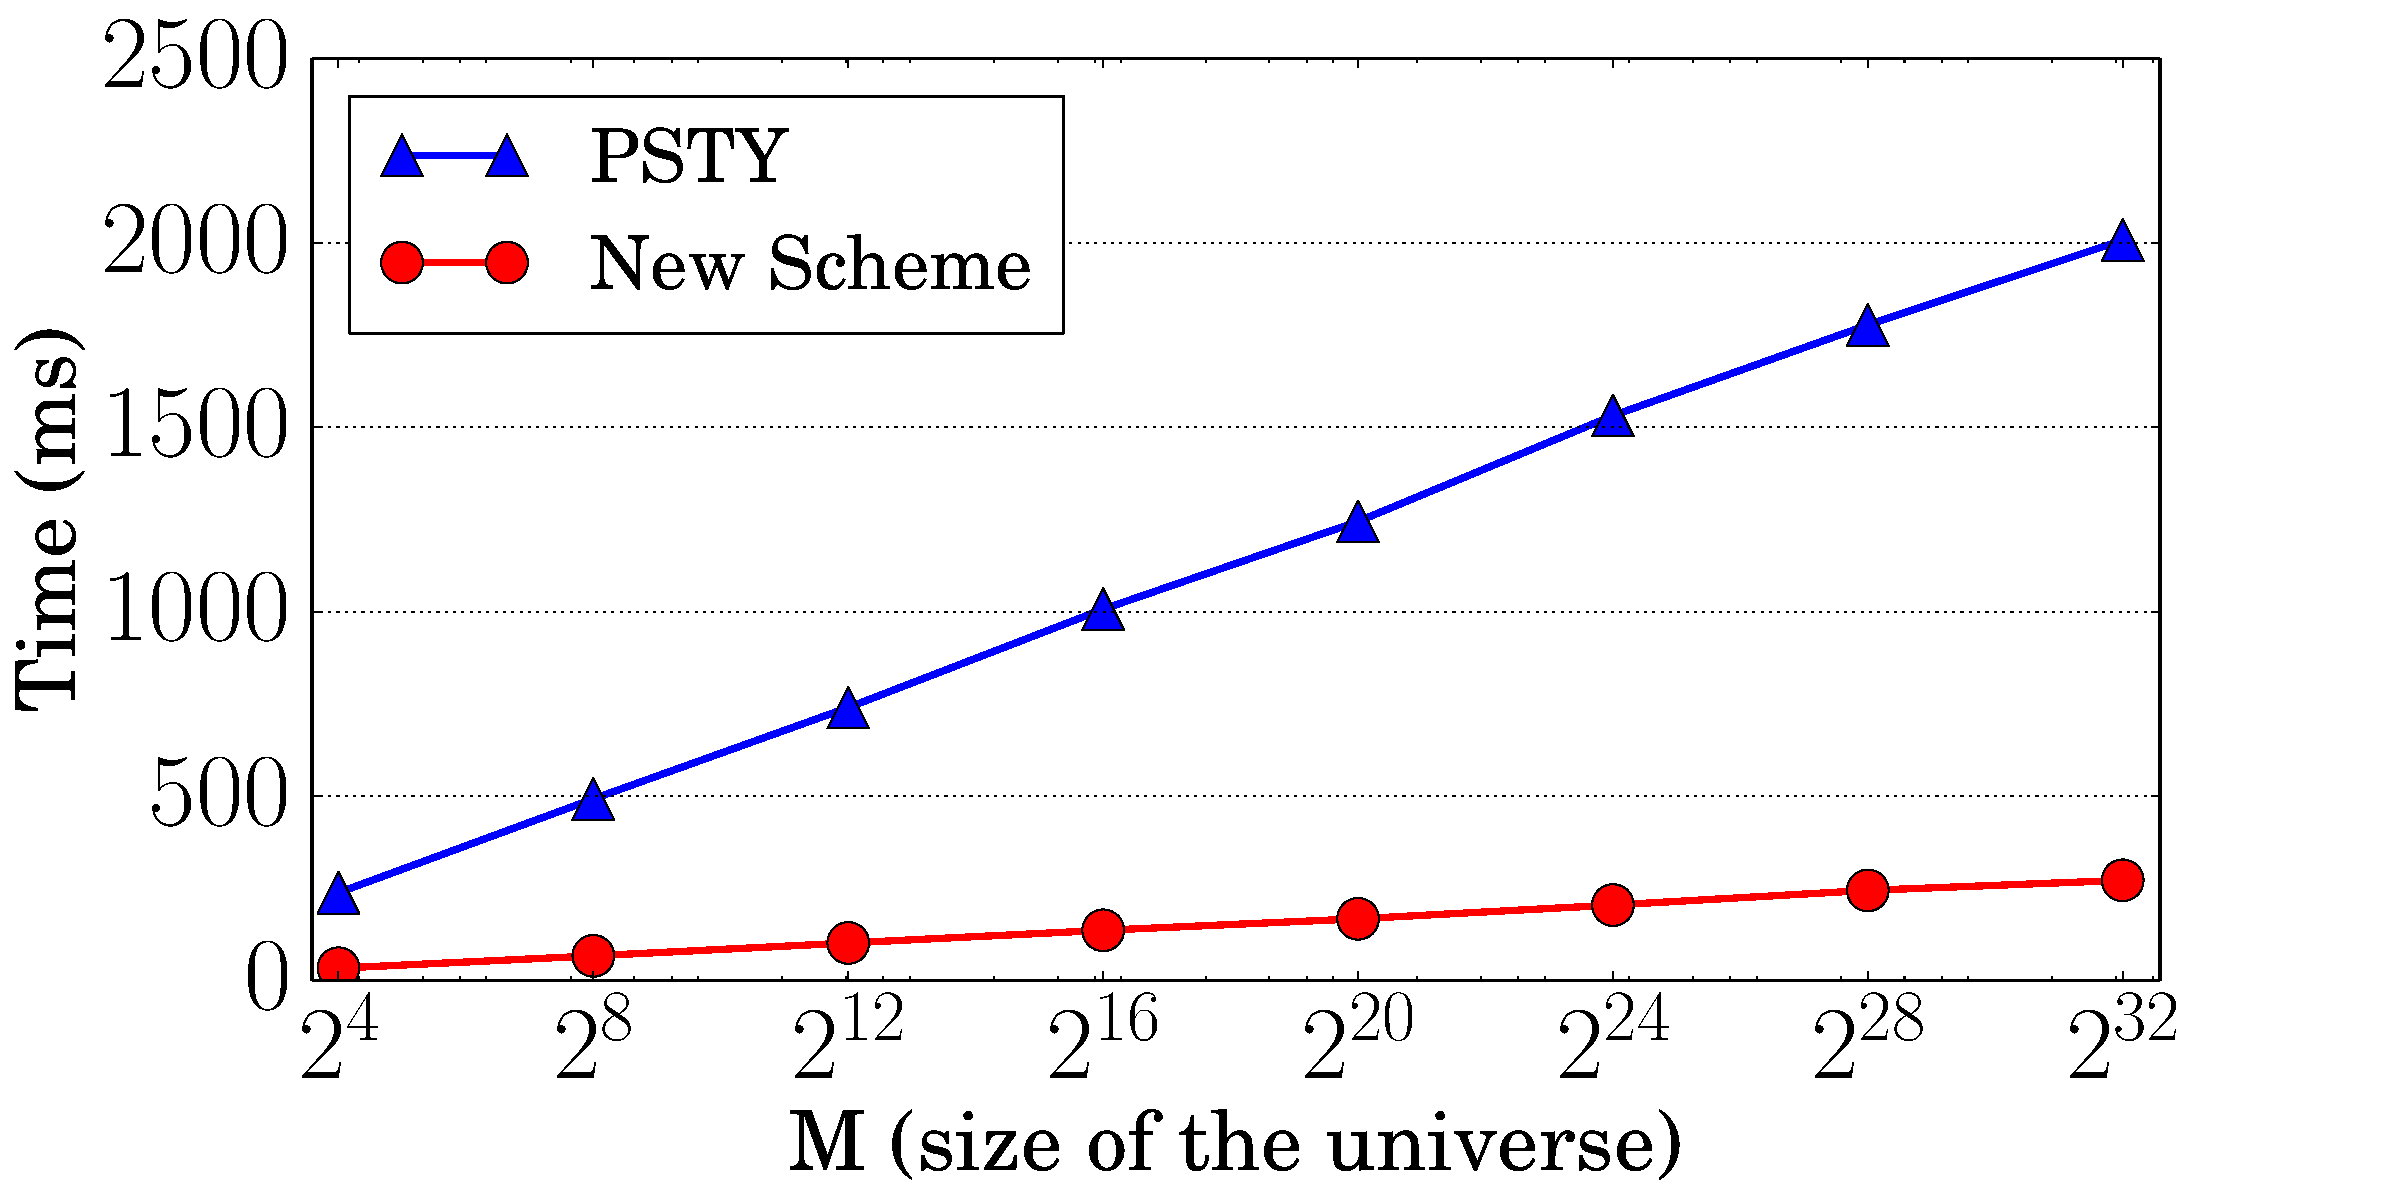
\includegraphics[scale = 0.23]{fig/verifytime_1.pdf}
\caption{Verification time. The $x$ axis is the size of universe $|M|$ in $\log$ scale. The size of stream is fixed to $n = 2^{32}$. The new scheme with $h_{new}$ achieves $7.5\times$ speed up.}\label{verify_time}
\end{minipage}\hfill
\begin{minipage}[t]{.49\textwidth}
\centering
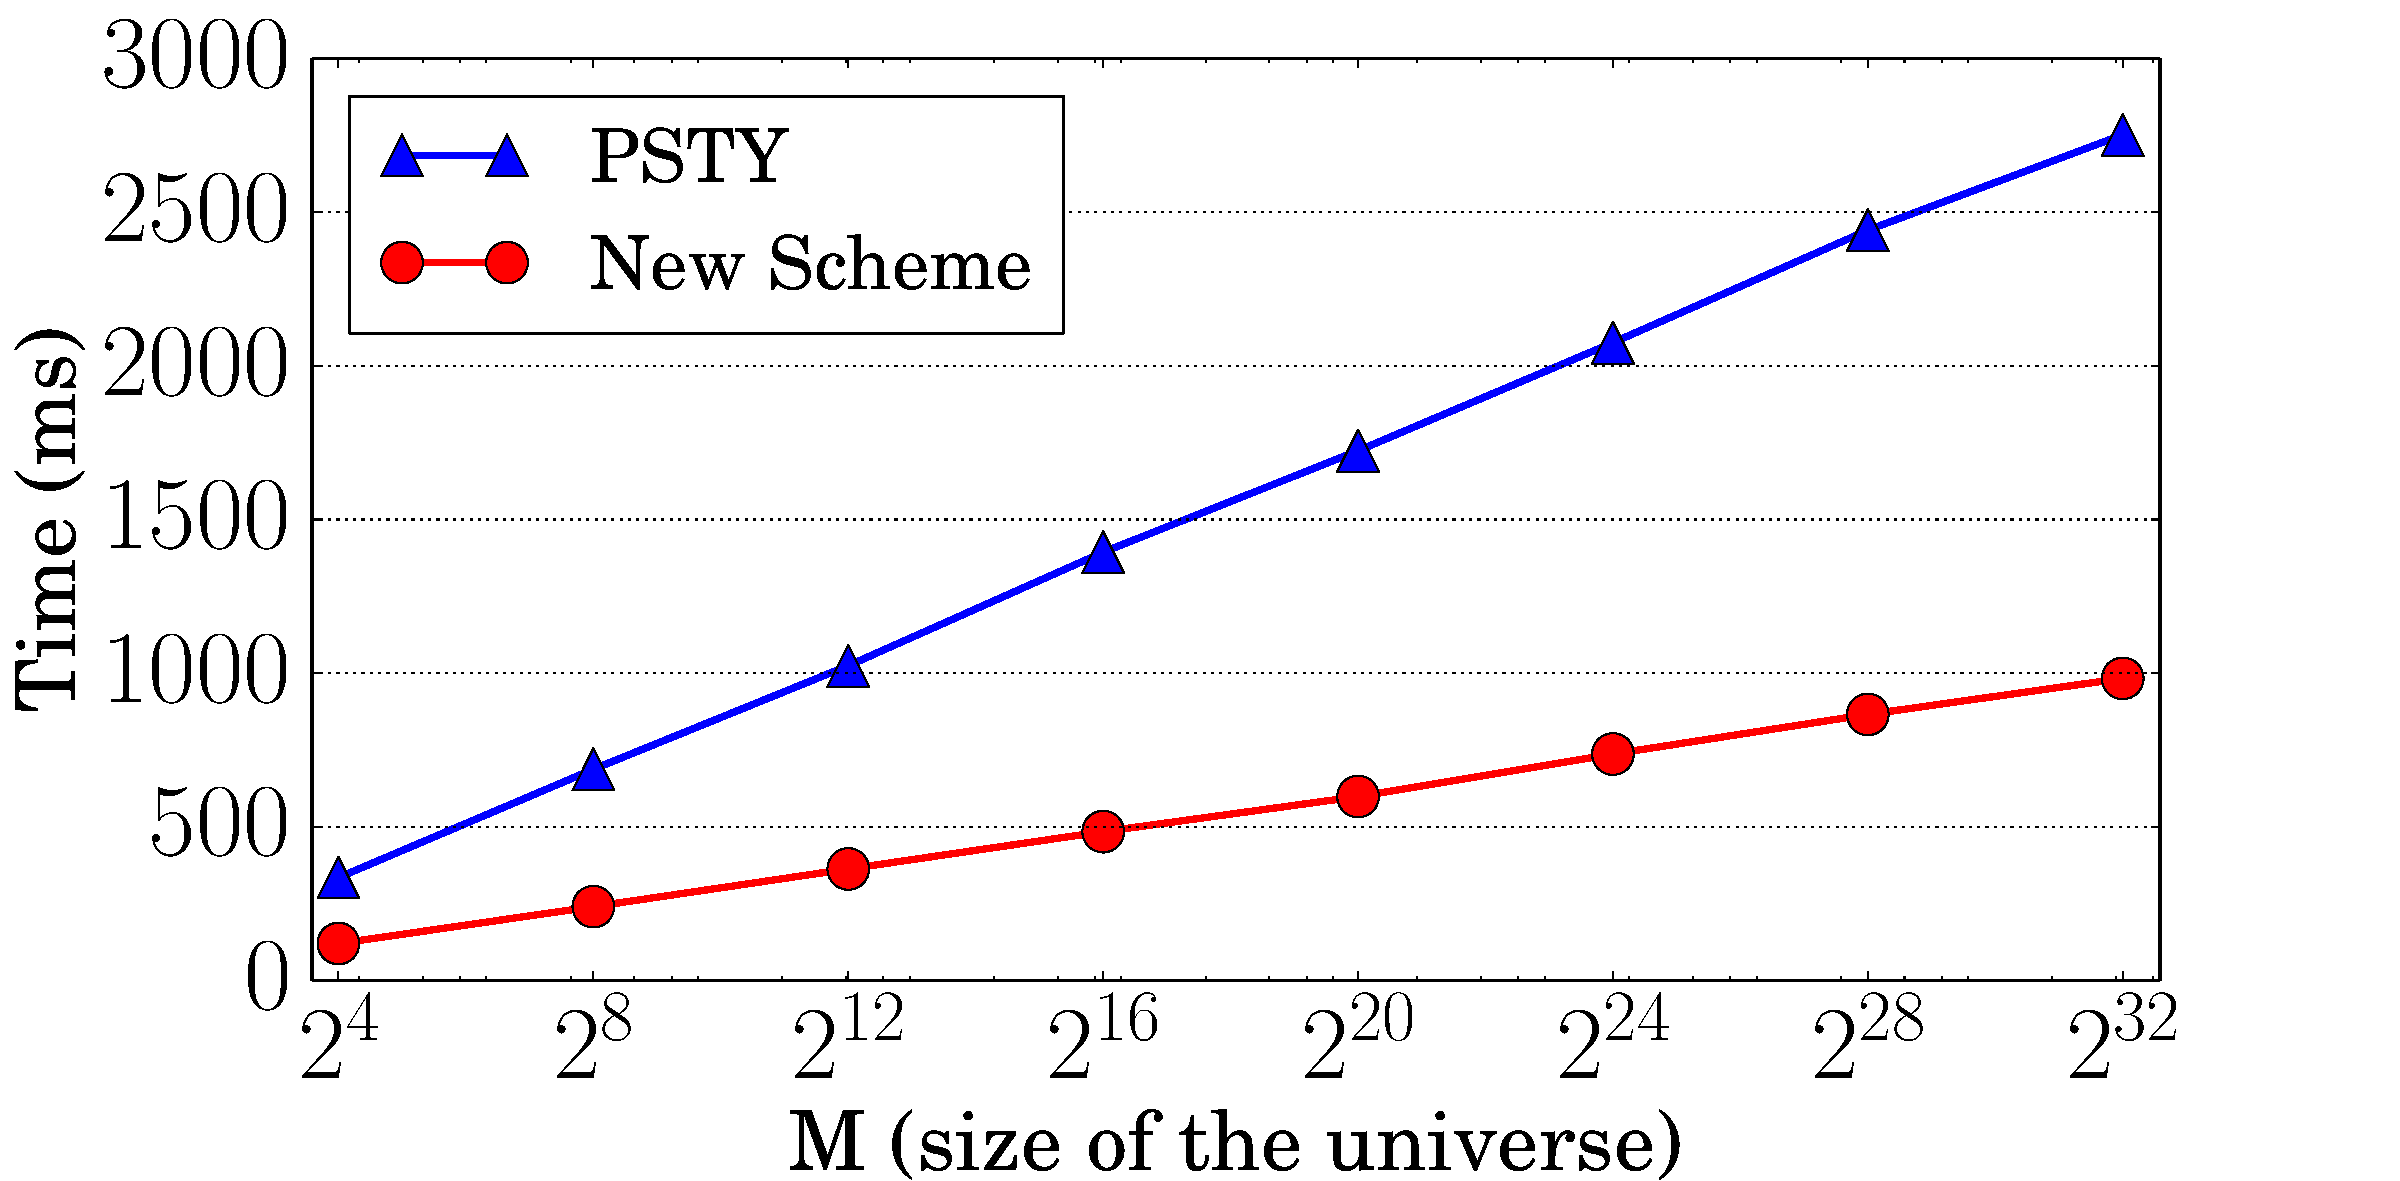
\includegraphics[scale = 0.23]{fig/updatetime_1.pdf}
\caption{Update time (client side).  The $x$ axis is the size of universe $|M|$ in $\log$ scale. The size of stream is fixed to $n = 2^{32}$. The new scheme with $h_{new}$ achieves $2.8\times$ speed up.}\label{update_time}
\end{minipage}\hfill
\end{figure*}


We implement the instantiations of our abstract SADS with both the hash function $h_{old}$ in PSTY~\cite{DBLP:conf/eurocrypt/PapamanthouSTY13} and our new GCK based hash function $h_{new}$ introduced in Section~\ref{new_hash}. We conduct a series of comparing experiments of these two instantiations. We show major performance improvements due to the GCK hash function.
\ignore{
First, we compare the performance of $h_{old}$ and $h_{new}$ in terms of the running time and key size. Next, we discuss the experimental results on all $6$ algorithms of Figure~\ref{algorithms_sads} by both instantiations. In particular, we present the empirical performance of \emph{verification}, \emph{update} and \emph{range search query} by the two instantiations.  }

{First, we highlight the asymptotic improvement of $h_{new}$ compared to $h_{old}$ in terms of the running time and key size. Next, we discuss the experimental results on various algorithms of Figure~\ref{algorithms_sads} for both instantiations. In particular, we present the empirical performance of \emph{verification}, \emph{update} and \emph{range search query} by the two instantiations.}


\vspace{1.5mm}\noindent{\bf Experiment setup.} The two instantiations are implemented in Mathlab 2014Ra and executed on a Windows 8.1 Desktop with 16GB of RAM.  The same data samples randomly generated are used in all experiments. We collected 10 runs for each data point and report the average.

There are two critical parameters involved in the experiments: 
\begin{enumerate}
\item The size of the stream $n$. This determines the parameter configuration of our GCK hash function $h_{new}$ by Algorithm~\ref{config_alg}. In particular, the running time and the key size of both $h_{new}$ and $h_{old}$ increase with respect to $n$. 
\item The size of the universe $M$. $|M|$ determines the size of the generalized hash tree (the generalized hash tree has $\log M$ layers), and consequently affects the running time of the query, update and verification of the SADS.
\end{enumerate}

\begin{table}[h!]\centering
%\caption{Detail statistics for $n=2^{32}$ and $|M| = 2^{32}$.}\label{asymptotic}
\caption{Asymptotic comparison between $h_{old}$ and $h_{new}$. Notice $t = \nu \log q$.}\label{asymptotic}
\begin{tabular}{|c|c|c|}

\hline
{}&running time&key size\\
\hline
PSTY&$O(\nu^2\log q)$&$O(\nu^2\log q)$\\
\hline
New Hash Function&$O(k\log k\log p)$&$O(k\log p)$\\
\hline

\end{tabular}
\end{table}


{
\vspace{1.5mm}\noindent{\bf Asymptotic comparison.} Table~\ref{asymptotic} shows the asymptotic complexity comparison of running time of hash functions and key size between $h_{old}$ and $h_{new}$\footnote{PSTY~\cite{DBLP:conf/eurocrypt/PapamanthouSTY13} has a set of different notations for parameters.}. As it is shown in both Section~\ref{instantiation} and PSTY~\cite{DBLP:conf/eurocrypt/PapamanthouSTY13}, the hash function $h_{old}$ is a matrix--vector multiplication, of which the running time is $O(\nu^2\log q)$ and the key size is the size of the matrix, $O(\nu^2\log q)$. The hash function $h_{new}$ constructed in Section~\ref{gck} is primarily based on polynomial multiplication, of which the running time using FFT is $O(k\log k\log p)$ and the key size is $O(k\log p)$. 

We generate parameters (e.g. $k$, $p$ and $q$) according to the size of the stream $n$ to ensure approximately the same security parameter ($100^+$ in both cases). In practice, $k$ is much smaller than $\nu$ and $\log p$ is roughly equal to $\log q$. Consequently, the improvement is rather significant.

\vspace{1.5mm}\noindent{\bf Running time of the hash functions.} Figure~\ref{hashtime} shows the running time of hashing one message by both $h_{old}$ and $h_{new}$ with increasing $n$. Our new hash function $h_{new}$ turns to outperform $h_{old}$ by orders of magnitude. Specifically, $h_{new}$ runs $1.6 \times$ faster when $n = 2^4$, and $9.8\times$ faster when $n = 2^{32}$, than $h_{old}$. This matches the asymptotic complexity comparison mentioned above. More importantly, the time cost of $h_{new}$ doesn't grow much as $n$ increases while it grows quasi-linearly with $n$ for $h_{old}$. As a result, the new hash function $h_{new}$ supports much larger streaming volume than $h_{old}$. 
%\babis{I want to cry with $h_{old}$ and $h_{new}$, PLEASE FIX THE NOTATION}

\begin{figure*}[Ht!]
\centering
\begin{minipage}[t]{.49\textwidth}
\centering
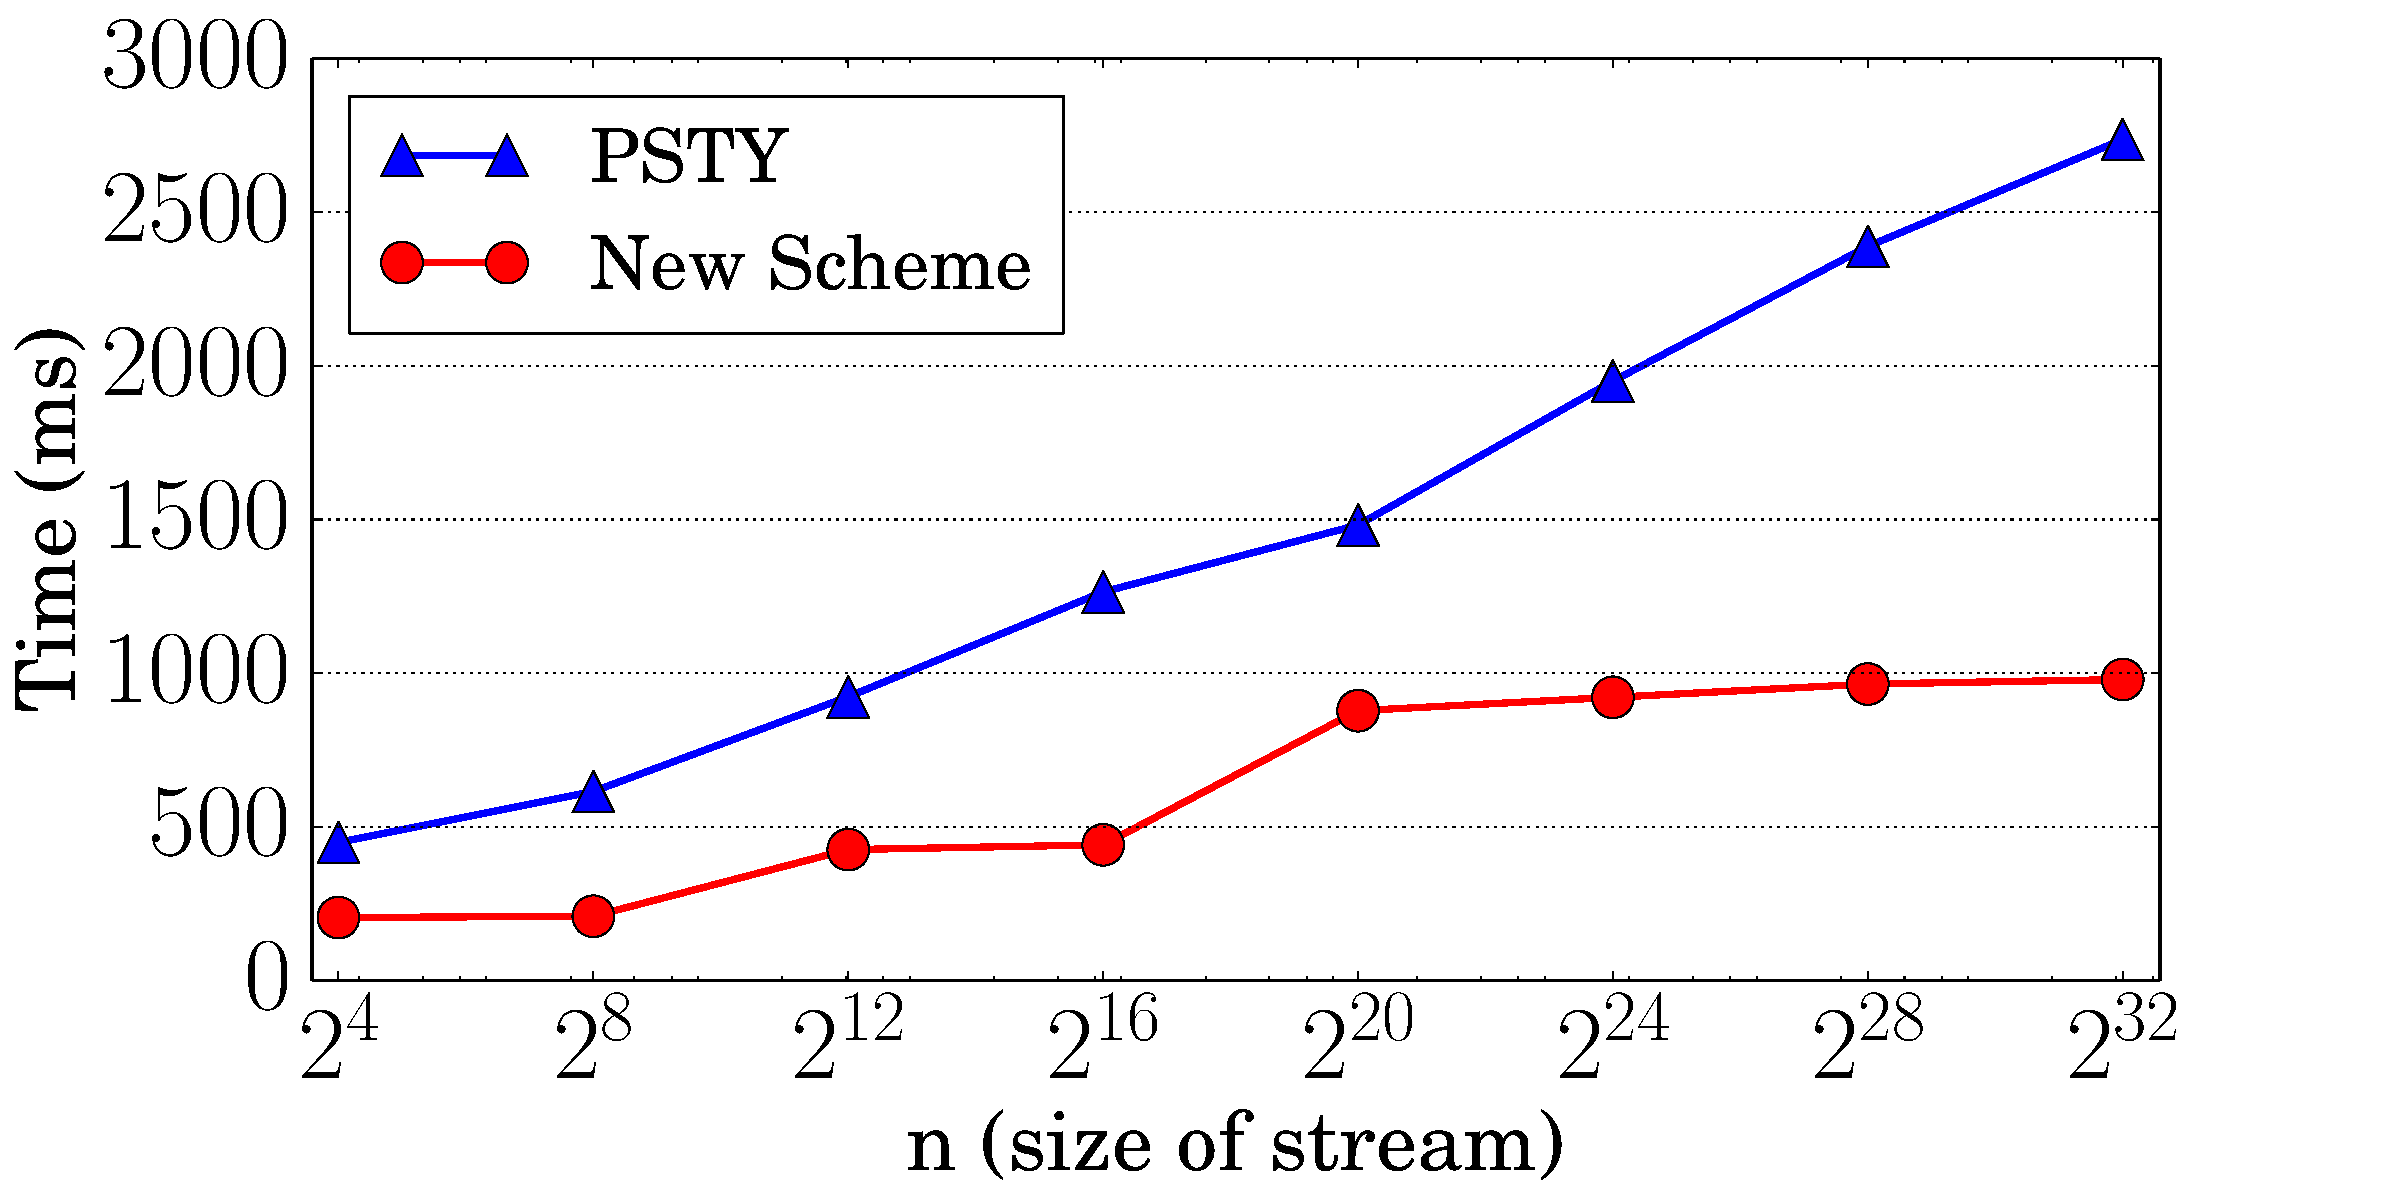
\includegraphics[scale = 0.23]{fig/updatetime_2.pdf}
\caption{Update time (client side). The $x$ axis is the size of stream $n$ in $\log$ scale. The size of the universe is fixed to $|M| = 2^{32}$. The new scheme with $h_{new}$ is $1.7\times$ faster when $n=2^4$, and $3.0\times$ faster when $n=2^{32}$, than the scheme with $h_{old}$.}\label{update_time2}
\end{minipage}\hfill
\begin{minipage}[t]{.49\textwidth}
\centering
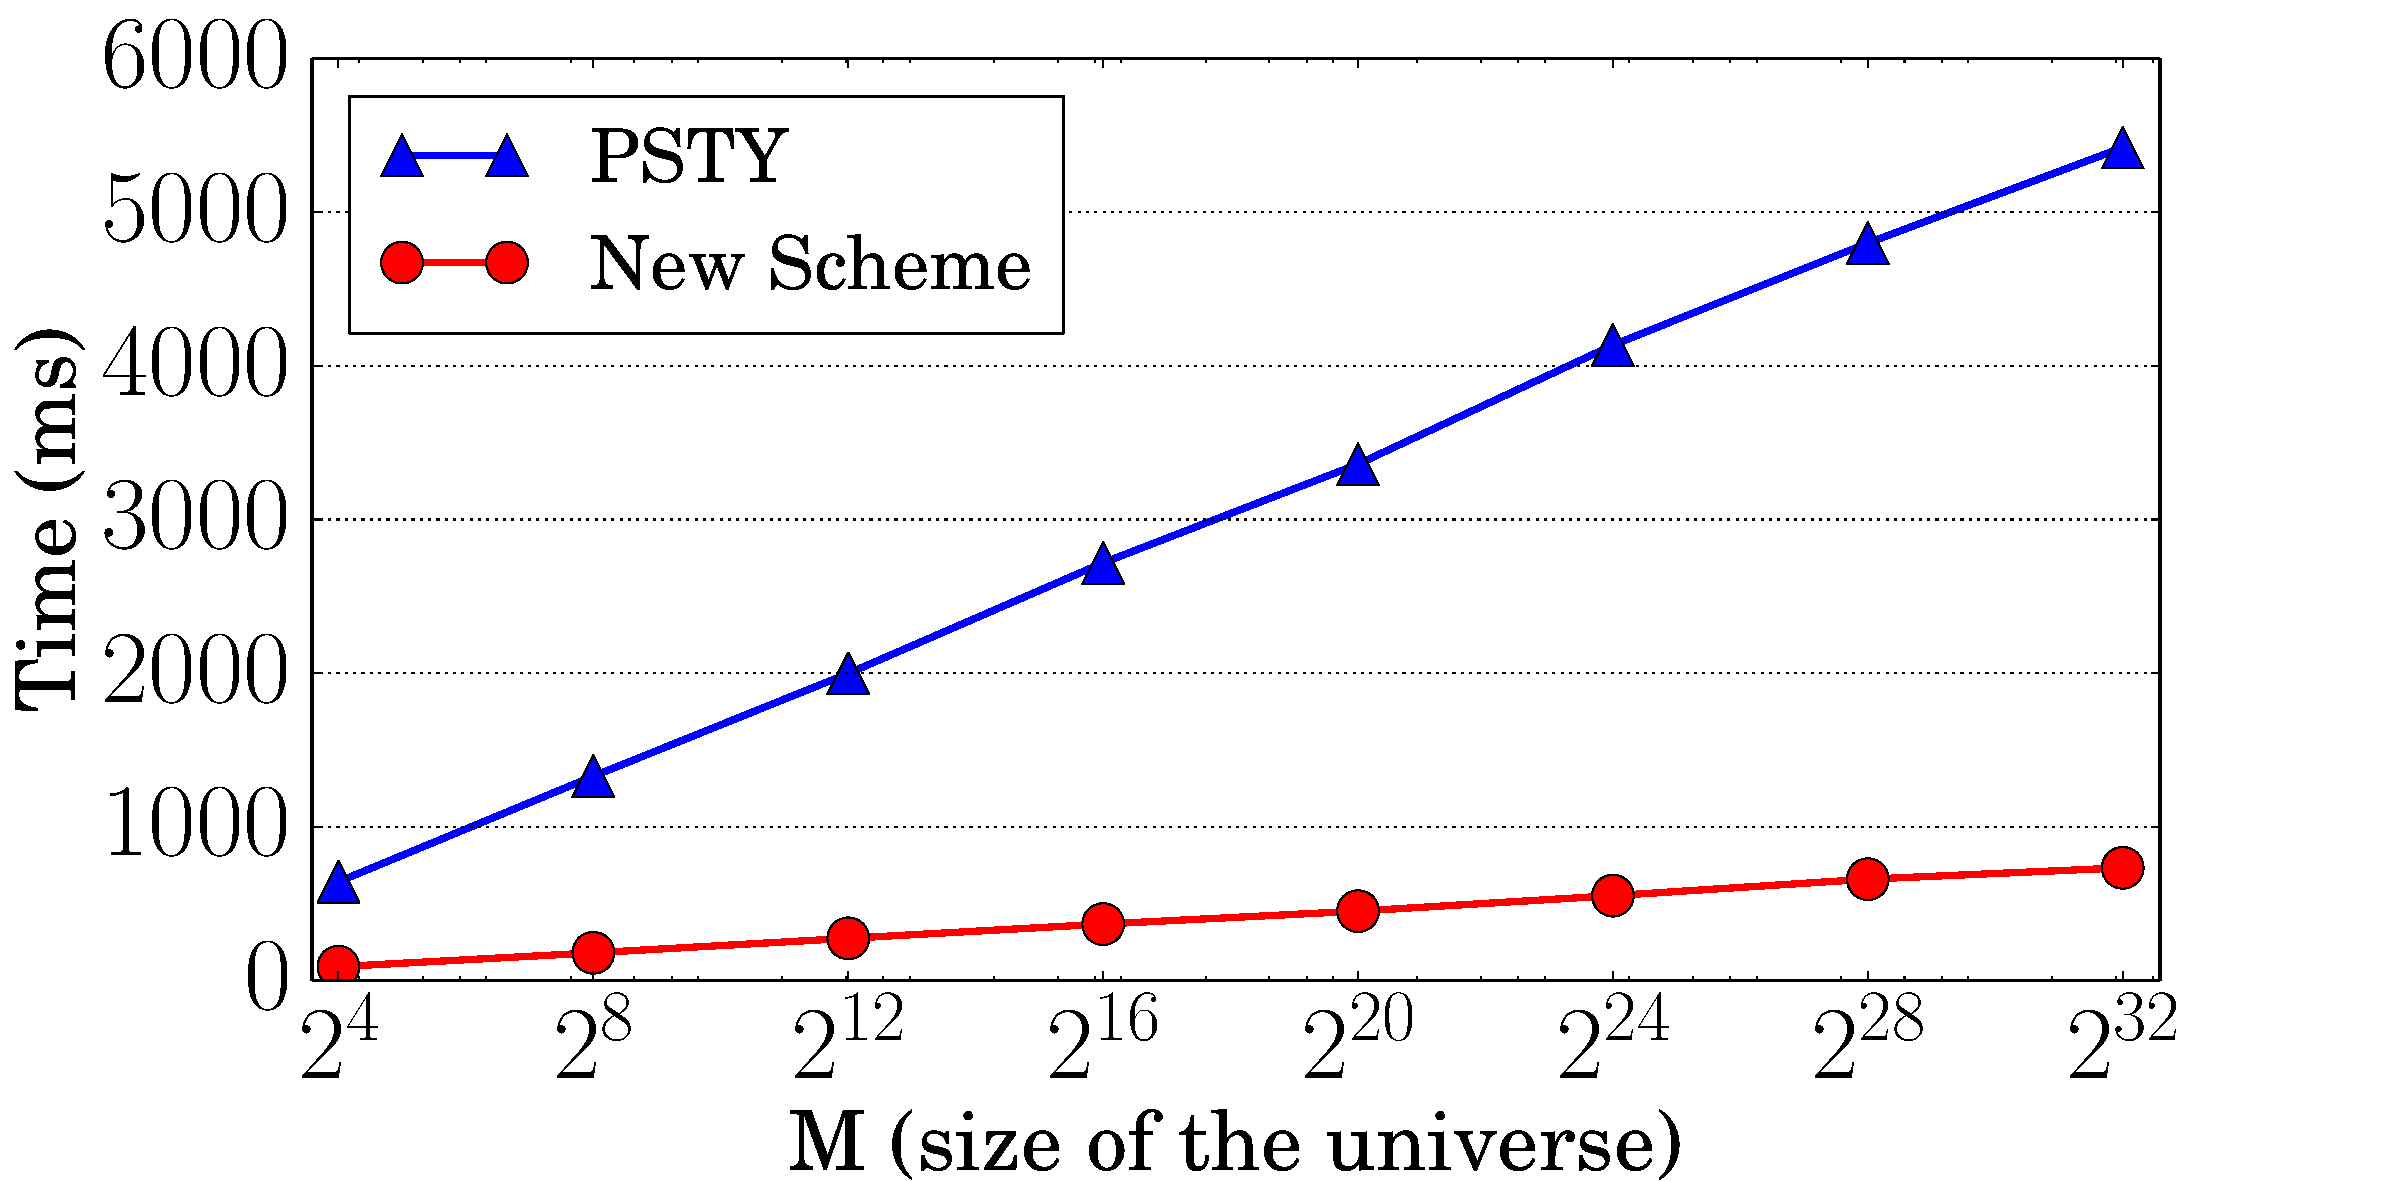
\includegraphics[scale = 0.23]{fig/range_search_1.pdf}
\caption{Range search time. The $x$ axis is the size of universe $|M|$ in $\log$ scale. The size of stream is fixed to $n = 2^{32}$. The new scheme with $h_{new}$ achieves $7.4\times$ speed up.}\label{range_time}
\end{minipage}\hfill
\end{figure*}


\vspace{1.5mm}\noindent{\bf Key size of hash functions.} Figure~\ref{keysize} shows the key sizes of both $h_{old}$ and $h_{new}$ with increasing $n$, which is plotted in $\log$-$\log$ scale. The key size of our new hash $h_{new}$ is only $0.73\%$ of the one of $h_{old}$ when $n = 2^4$, and $0.077\%$ of the ones of $h_{old}$ when $n = 2^{32}$. This significant improvement is due to the advantages of circular lattices over regular lattices. Moreover, the key size of $h_{new}$ grows roughly linearly with $n$ while it grows quadratically with $n$ for $h_{old}$. Notice the public key of the abstract SADS is the key of the two hash functions ${\bf {\cal H}_{L}}$, ${\bf {\cal H}_{R}}$. Hence, the improvement of hash function key size in Figure~\ref{keysize} applies directly to the public key size of the entire scheme.%\babis{the last two statements are not clear}
}

\vspace{1.5mm}\noindent{\bf Preprocessing.} In algorithms $\mathsf{initialize}()$ of Figure~\ref{algorithms_sads}, the digest and every node labels of the generalized hash tree are initialized to be $\bf 0$s. Hence, the preprocessing time is independent of the hash function choice.
Notice that in our implementations, the generalized hash tree is dynamically allocated, and the storage cost is proportional to the nonzero values stored in the leaves. In this way, we can run the experiments on a large universe of size up to $|M| = 2^{32}$.

\vspace{1.5mm}\noindent{\bf Proof Computation.} The server needs to compute the result along with a proof, responding to a query from the verifier. We discuss two ways to compute the proof on the server side. (1) The server constructs and stores the whole generalized hash tree, and returns the corresponding labels of nodes required by the proof. (2) The server only stores the values in the leaves of the generalized hash tree, and computes labels of nodes for a proof each time. There is a time-space trade-off between these two approaches. We choose the former in our implementations, in which case the proof computation is just an index searching and returning procedure. Hence, the proof computation time is the same for both instantiations. 

\vspace{1.5mm}\noindent{\bf Verification.} Figure~\ref{verify_time} shows the comparison for verification time by the instantiation with $h_{new}$ and the instantiation with $h_{old}$. The $x$ axis is the size of the universe $M$. The upper bound of the streaming $n$ is fixed to $2^{32}$. As we can see, the instantiation with our new hash function $h_{new}$ outperforms the instantiation with $h_{old}$ dramatically. Specifically, the verification time of the new instantiation with $h_{new}$ is 7.5 times faster than the one with $h_{old}$. Moreover, Figure~\ref{verify_time} shows that the verification time grows on the order of $O(\log M)$, matching what the algorithm $\mathsf{verify}()$ indicates. Finally, the verification time is only $10\sim100$ milliseconds with $h_{new}$, which makes the new scheme practical.


\vspace{1.5mm}\noindent{\bf Update.} Figure~\ref{update_time} shows that the instantiation with $h_{new}$ runs 2.8 times faster than the one with $h_{old}$ for the client side update. Notice that the client side update and the server side update go through the same computations, except that the server also updates the labels of nodes along the verification path. Therefore, the time cost of the client side update and the server side update is roughly the same. We omit the comparison for the server update time here. Moreover, the update time grows logarithmically with $M$ as desired in Figure~\ref{update_time}.

In practice, the size of the universe $|M|$ is usually fixed for a certain streaming application. To illustrate such scenario, we show the update time as $n$ increases, with $|M|$ fixed to $2^{32}$. Figure~\ref{update_time2} shows that the instantiation with $h_{new}$ is $1.7\sim3.0$ times faster than the one with $h_{old}$. The larger streaming volume $n$ results in the more significant improvement in terms of update time.



\vspace{1.5mm}\noindent{\bf Range search.} The range search functionality is implemented and the results are shown in Figure~\ref{range_time}. The range search time cost of both instantiations is slightly larger than two times of their verification time cost, and hence grows logarithmically with $M$ as desired.
Moreover, the range search of the instantiation with $h_{new}$ is 7.4 times faster than the one with $h_{old}$.

\begin{table}[h!]\small
\caption{Detail statistics for $n=2^{32}$ and $|M| = 2^{32}$.}\label{data}
\begin{tabularx}{0.48\textwidth}{p{1.2cm}|c|c|c|c|c}
%\begin{tabular}{|c|c|p{0.9cm}|p{1.2cm}|p{0.6cm}|p{0.9cm}|}
%\begin{tabular}{|c|c|c|c|c p{0.6cm}|c|}
\hline
{}&running&key size&verification&update&range\\
%\hline
{}&time (ms)&(MB)&(s)&(s)&search (s)\\
\hline
Instantiation&\multirow{2}{*}{2.74}&\multirow{2}{*}{0.21}&\multirow{2}{*}{0.27}&\multirow{2}{*}{0.98}&\multirow{2}{*}{0.73}\\
with $h_{new}$&&&&&\\
\hline
Instantiation&\multirow{2}{*}{26.84}&\multirow{2}{*}{265.02}&\multirow{2}{*}{2.01}&\multirow{2}{*}{2.75}&\multirow{2}{*}{5.42}\\
with $h_{old}$&&&&&\\
\hline

\end{tabularx}
\end{table}

%\yi{Please update the caption/legend in the figures accordingly. Use instantiation with $h_{new}$ and instantiation with $h_{old}$ .}

Finally, Table~\ref{data} shows the statistics for both instantiations when $n=2^{32}$ and $|M|=2^{32}$. We can see that hashing a message by $h_{new}$ only takes 2.74 milliseconds while \emph{update}, \emph{verification} and \emph{range search} of the new instantiation with $h_{new}$ all takes less than one second. Meanwhile, the key size of the new scheme is only 0.21MB, which is practical to store and manage, to the key of $h_{old}$ which is 265MB.

